\begin{definition}
\emph{(Optimierungsprobleme mit linearen Gleichungsnebenbedingungen)}
\begin{align}
  \min_{x \in \R^n}\ & f(x) \tag{PLG}\label{prob:opt_prob_mit_lin_gl_nebenbed}\\
              \nb & Ax = b \notag
\end{align}
$A$ sei eine $(m \times n)$-Matrix und $b$ sei ein Vektor mit $m$ Elementen.
\end{definition}

D.\,h., die Menge $\F$ sieht hier so aus:  $\F = \{ x \in \R^n\ |\ A x = b \}$.

\begin{example}\label{example:opt_prob_mit_lin_gl_nebenbed}
Ein einfaches Beispiel eines
Optimierungsproblems~\eqref{prob:opt_prob_mit_lin_gl_nebenbed} ist
\begin{equation}
\begin{split}
  \min_{x \in \R^2}\ & x_1^2 + x_2^2 \\
  \nb & x_1 + x_2 = 1.
\end{split}
\end{equation}
Die zul�ssigen Punkte dieses Problems liegen auf einer Gerade
(siehe Abbildung~\ref{fig:beispiel_opt_prob_mit_lin_gl_nebenbed}).
\end{example}
\begin{figure}[h]
\centering
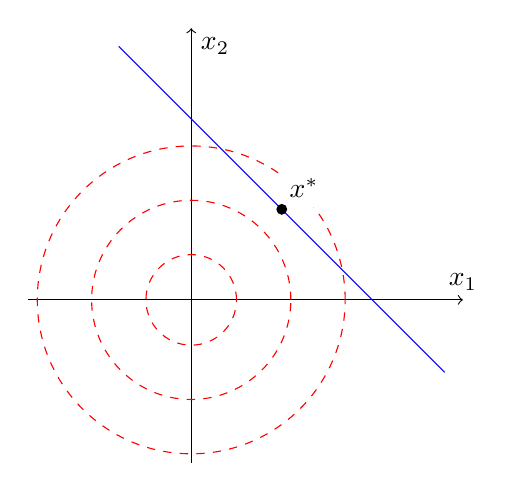
\begin{tikzpicture}[scale=2.3]
  \draw[->] (-0.9,0) -- (1.5,0) node [above] {$x_1$};
  \draw[->] (0,-0.9) -- (0,1.5) node [below right] {$x_2$};
  % Die Niveaulinien
  \foreach \r in {0.25, 0.55, 0.85}
    \draw[dashed,color=red] (0,0) circle (\r);
  % Schreibe x*
  \draw (0.49,0.51) node [above right,fill=white] {$x^*$};
  % Die Nebenbedingung
  \draw[color=blue] (-0.4,1.4) -- (1.4,-0.4);
  \draw (1,0.05) node [above] {$\F$};
  % Der Kreis f�r x*
  \fill (0.5,0.5) circle (0.03);
\end{tikzpicture}
\caption{Geometrische Darstellung
des Beispiels~\ref{example:opt_prob_mit_lin_gl_nebenbed}}
\label{fig:beispiel_opt_prob_mit_lin_gl_nebenbed}
\end{figure}

\begin{theorem} \label{satz:notw_bed_fuer_prob_mit_lin_gl_nebenbed}
\emph{(Notwendige Bedingung, vgl. Satz 5.3.2 in \cite[S.~174]{alt})}\\
Sei $\xopt$ eine lokale L�sung des
Problems~\eqref{prob:opt_prob_mit_lin_gl_nebenbed}
und $f$ sei in $\xopt$ differenzierbar.
Dann gibt es ein $\lambda \in \R^m$ mit
\begin{equation}
  \nabla f(\xopt) + A^T \lambda = 0.
\end{equation}
Hat A einen vollen Rang, dann ist $\lambda$ eindeutig bestimmt.
\end{theorem}

Diese Bedingung hei�t die Multiplikatoren-Regel von Lagrange und
man bezeichnet $\lambda$ als Lagrange-Multiplikator.

\begin{theorem}
\emph{(Hinreichende Bedingung, vgl. Satz 5.3.8 in \cite[S.~177]{alt})}\\
Sei $f$ in $\xopt$ zweimal stetig differenzierbar. Die notwendige Bedingung
in Satz~\ref{satz:notw_bed_fuer_prob_mit_lin_gl_nebenbed} sei erf�llt.
Es existiere eine Konstante $\alpha > 0$ mit
\begin{equation}
\label{eq:hesse_matrix_pos_def_auf_kern_A}
  d^T f''(x) d \geq \alpha \|d\|^2 \qquad \forall d \in \kr A.
\end{equation}
Dann ist $\xopt$ eine strikte L�sung des
Problems~\eqref{prob:opt_prob_mit_lin_gl_nebenbed}.
\end{theorem}

Eine wichtige Grundlage zum L�sen des
Problems~\eqref{prob:opt_prob_mit_lin_gl_nebenbed}
als unrestringiertes Problem
ist die Definition der Nullraum-Matrix
(vgl. \cite[S.~182]{alt}).

\begin{definition}
\label{def:nullraum_matrix}
\emph{(Nullraum-Matrix)}\\
Eine $(n \times s)$-Matrix $Z$ hei�t Nullraum-Matrix von~$A$, wenn f�r $d \in
\R^n$ gilt
\begin{equation}
d \in \kr A \quad \Leftrightarrow \quad d = Z z \text{ f�r ein } z \in \R^s.
\end{equation}
D.\,h. $\im Z = \kr A$.
\end{definition}

Sei $w$ eine L�sung der Gleichung $Ax=b$.
Man kann nun die Menge $\F$ des Problems~\eqref{prob:opt_prob_mit_lin_gl_nebenbed}
so schreiben:
\begin{equation}
  \F = w + \kr A = w + \im Z = w + \{ Z z\ |\ z \in \R^s \}.
\end{equation}

D.\,h., jedes Element $x \in \F$ ist mit $w + Zz$, $z \in \R^s$, zu ersetzen.
Das Problem~\eqref{prob:opt_prob_mit_lin_gl_nebenbed} ist dann �quivalent zu
\begin{equation}
  \label{prob:opt_prob_unrestr_mithilfe_nullraum_matrix}
  \min_{z \in \R^s} F(z) := f(w + Zz).
\end{equation}

Dieses Problem hat keine Nebenbedingung mehr, ist also unrestringiert.
Man kann folglich Verfahren f�r unrestringierte Probleme anwenden.
